% ===========================================================================
% Section 6 -- Comparative computational evaluation
% ===========================================================================

\subsection{Setup and fairness}

(CF+) and (SP-CG) were run on the same 76 instances as the baseline, on the
same machine, with the same solver (HiGHS 1.16, default parameters), one
thread per run, five runs in parallel and the same limit of 300\,s per run
(\texttt{results/raw/improved.csv}). For (SP-CG), the 300\,s include
everything: greedy, column generation, price-and-branch, enumeration and the
final MILP. Each (CF+) component was also switched off in turn on the 15
scale instances with $40\le n\le100$ (\texttt{results/raw/ablation.csv}).
Tables and figures are generated by \texttt{src/analyze\_improved.py}.

A run counts as \emph{solved} only if it proves optimality for the problem
itself. (CF)-type models (CF, CF-M, CF+) are therefore counted as solved only
on transitive instances; on the others they solve a restriction
(Section~\ref{sec:compact}). Unsolved runs count with 300\,s.

\paragraph{Correctness.} The validator accepted all 396 solutions of the
baseline and the new runs. On every instance where several methods prove
optimality, they report the same value. On the non-transitive instances
(SP-CG) always matches (AF) where (AF) is solved, while the (CF)-type
models are up to $0.6$ above the optimum on the arc\_drop instances, and
(CF+) is $3.0$ above it on \texttt{csp50} ($20.4$ against $17.4$, i.e.\ 17\%).
This confirms the theory: the restriction can cost a lot.

While developing (SP-CG) we found two problems that would have corrupted the
comparison, and we report them because they matter for reproducibility.
First, the MIP start of HiGHS~1.16 can produce wrong ``optimal'' values
(Section~\ref{sec:cfp}); we use the improving cut instead. Second, on MILPs
with more than half a million columns HiGHS exceeded the time limit by up to
three minutes; we therefore cap the enumeration at 250\,000 columns, above
which the remaining time goes to price-and-branch. With this cap, no
(SP-CG) run exceeds 301\,s.

\subsection{Overall results}

\begin{table}[ht]
\centering
\small
\caption{All 76 instances. Solved: optimality proved (see the fairness rule).
Shifted geometric mean of the time with shift 1\,s. Primal gap: distance of
the solution found from the best known solution (the best over all runs),
100\% when no solution was found.}
\label{tab:cmp-summary}
\begin{tabular}{lrrrrr}
\toprule
Model & solved & too large & mean time [s] & shifted geo.\ mean [s] & primal gap \% \\
\midrule
(AF) & 15/76 & 12 & 245 & 140.3 & 27.4 \\
(CF) & 47/76 & 14 & 120 & 19.6 & 19.5 \\
(CF-M) & 41/76 & 12 & 169 & 65.5 & 20.4 \\
(CF+) & 49/76 & 5 & 112 & 19.4 & 10.1 \\
(SP-CG) & 70/76 & 0 & 25 & 1.1 & 0.0 \\
\bottomrule
\end{tabular}

\end{table}

Table~\ref{tab:cmp-summary} and Figure~\ref{fig:cmp-profile} summarise the
comparison. (SP-CG) solves 70 of the 76 instances, against 47 for the best
baseline model (CF), and is about 18 times faster in shifted geometric mean
(1.1\,s against 19.6\,s). It is never too large and finds the best known
solution on all 76 instances. In the performance profile it is the fastest
method on every instance solved by any method. (CF+) improves (CF) only
moderately: 49 solved instead of 47, a slightly lower mean time, and,
because it can be built for much larger instances and starts from the greedy
solution, a primal gap of 10\% instead of 20\%.

\begin{figure}[ht]
\centering
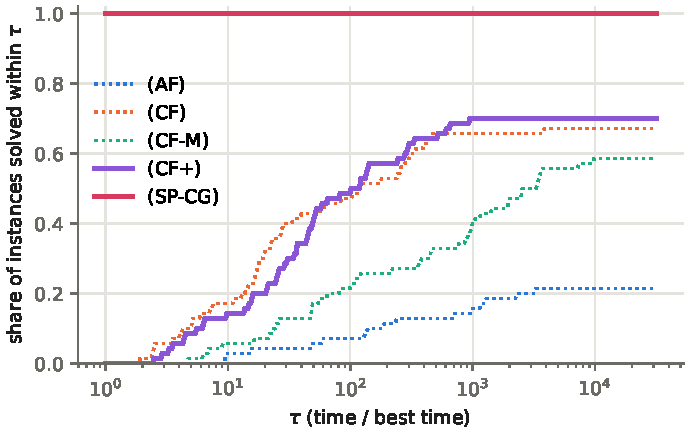
\includegraphics[width=0.62\textwidth]{figures/cmp_profile}
\caption{Performance profile (Dolan--Mor\'e) of the running time on the 70
instances solved by at least one method: share of instances that a method
solves within $\tau$ times the time of the fastest method.}
\label{fig:cmp-profile}
\end{figure}

\subsection{Scalability}

\begin{table}[ht]
\centering
\small
\setlength{\tabcolsep}{4pt}
\caption{Scale suite: instances solved (of 3 seeds) and mean time [s]
(300 for unsolved runs). ``large'': over 4 million non-zeros.}
\label{tab:cmp-scale}
\begin{tabular}{rrrrrrrrrrr}
\toprule
 & \multicolumn{2}{c}{(AF)} & \multicolumn{2}{c}{(CF)} & \multicolumn{2}{c}{(CF-M)} & \multicolumn{2}{c}{(CF+)} & \multicolumn{2}{c}{(SP-CG)} \\
\cmidrule(lr){2-3} \cmidrule(lr){4-5} \cmidrule(lr){6-7} \cmidrule(lr){8-9} \cmidrule(lr){10-11}
$n$ & solved & time & solved & time & solved & time & solved & time & solved & time \\
\midrule
10 & 3/3 & 0 & 3/3 & 0 & 3/3 & 0 & 3/3 & 0 & 3/3 & 0 \\
15 & 3/3 & 1 & 3/3 & 0 & 3/3 & 0 & 3/3 & 0 & 3/3 & 0 \\
20 & 3/3 & 4 & 3/3 & 0 & 3/3 & 1 & 3/3 & 0 & 3/3 & 0 \\
25 & 3/3 & 18 & 3/3 & 0 & 3/3 & 1 & 3/3 & 1 & 3/3 & 0 \\
30 & 2/3 & 124 & 3/3 & 4 & 3/3 & 62 & 3/3 & 16 & 3/3 & 0 \\
40 & 0/3 & 300 & 3/3 & 6 & 2/3 & 148 & 3/3 & 6 & 3/3 & 0 \\
50 & 0/3 & 300 & 3/3 & 5 & 3/3 & 142 & 3/3 & 7 & 3/3 & 0 \\
60 & 0/3 & 300 & 1/3 & 210 & 0/3 & 300 & 2/3 & 129 & 3/3 & 0 \\
80 & 0/3 & 300 & 1/3 & 220 & 0/3 & 300 & 2/3 & 133 & 3/3 & 1 \\
100 & 0/3 & 300 & 0/3 & 300 & 0/3 & 300 & 0/3 & 300 & 3/3 & 15 \\
150 & \multicolumn{2}{c}{large} & \multicolumn{2}{c}{large} & 0/3 & 300 & 0/3 & 300 & 3/3 & 1 \\
200 & \multicolumn{2}{c}{large} & \multicolumn{2}{c}{large} & \multicolumn{2}{c}{large} & 0/3 & 300 & 3/3 & 2 \\
\bottomrule
\end{tabular}

\end{table}

\begin{figure}[ht]
\centering
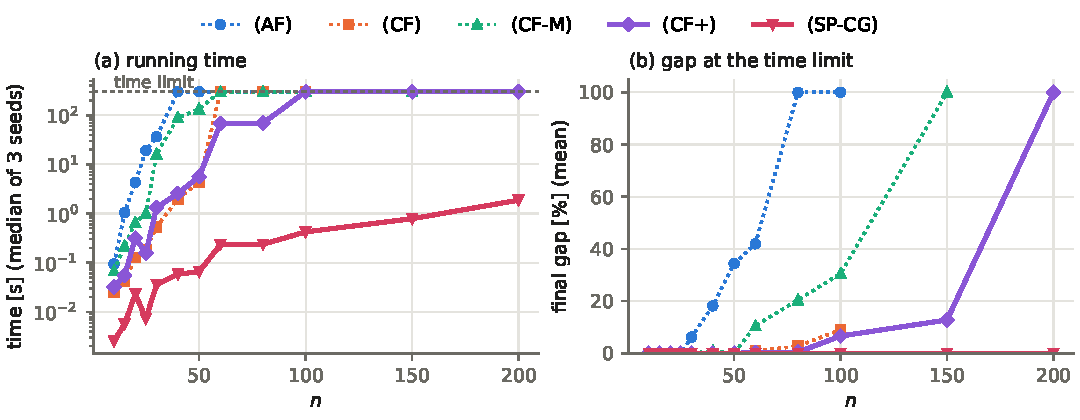
\includegraphics[width=\textwidth]{figures/cmp_scale}
\caption{Scale suite: (a) running time and (b) final gap against $n$;
dotted lines are the baseline models of Section~\ref{sec:baseline-exp}.}
\label{fig:cmp-scale}
\end{figure}

Table~\ref{tab:cmp-scale} and Figure~\ref{fig:cmp-scale} show how far each
method scales. The largest size solved for all three seeds goes from $n=50$
(CF) to $n=200$ (SP-CG), the largest size in the suite. At $n=200$ (SP-CG)
needs 2\,s; at $n=100$ its mean time (15\,s) comes from a single instance
that needed the enumeration (42\,s). (CF+) solves two of three seeds at
$n=60$ and $n=80$, where (CF) solves one, and can be built up to $n=200$,
but it does not solve any instance with $n\ge100$.

\subsection{Strength of the bounds}

\begin{table}[ht]
\centering
\small
\caption{Bounds on the 60 transitive instances with a known optimum $z^*$:
mean LP gap and root gap (for (SP-CG): $z_{\mathrm{LP}}$ and
$\lceil 5z_{\mathrm{LP}}\rceil/5$), median nodes of the solved runs, solved
runs.}
\label{tab:cmp-bounds}
\begin{tabular}{lrrrr}
\toprule
Model & LP gap \% & root gap \% & nodes (median) & solved \\
\midrule
(AF) & 19.6 & 12.4 & 1 & 14/60 \\
(CF) & 29.6 & 1.0 & 1 & 47/60 \\
(CF-M) & 29.5 & 7.4 & 1111 & 41/60 \\
(CF+) & 24.2 & 0.8 & 1 & 49/60 \\
(SP-CG) & 0.1 & 0.0 & 0 & 60/60 \\
\bottomrule
\end{tabular}

\end{table}

Table~\ref{tab:cmp-bounds} explains the gap between the two improvements.
The LP bound of (SP) is 0.1\% from the optimum on average, and it is equal
to the optimum on 64 of the 70 instances with a known optimum. This is far stronger than any
compact model, including (AF) (19.6\%), as predicted in Section~\ref{sec:sp}:
(SP) convexifies the per-employee constraints that the compact LPs satisfy
only on average. With such a bound, column generation alone usually proves
optimality: the enumeration was completed on only 7 instances. The clique rows
of (CF+) do strengthen its LP (24.2\% against 29.6\% for (CF)), but after
HiGHS's root cuts the difference almost vanishes (0.8\% against 1.0\%): the
solver's own clique cuts already recover most of it.

\subsection{OR-Library instances}

\begin{table}[ht]
\centering
\small
\setlength{\tabcolsep}{4pt}
\caption{OR-Library instances. Best baseline: (AF), the only exact baseline
model there. For (SP-CG): LP bound, final bound, best solution, total time
(TL: time limit), column generation time and number of enumerated columns
(--: enumeration not needed or abandoned).}
\label{tab:cmp-orlib}
\begin{tabular}{rrrrrrrrrr}
\toprule
 & & \multicolumn{2}{c}{best baseline} & \multicolumn{6}{c}{(SP-CG)} \\
\cmidrule(lr){3-4}\cmidrule(lr){5-10}
$n$ & greedy & obj & bound & $z_{\mathrm{LP}}$ & bound & obj & time [s] & CG [s] & enum.\ cols \\
\midrule
50 & 18.8 & 18.4 & 14.6 & 17.40 & 17.4 & 17.4 & 0 & 0.0 & -- \\
100 & 33.8 & 60.8 & 26.2 & 29.93 & 30.2 & 30.2 & 1 & 0.1 & 1009 \\
150 & 52.6 & 88.8 & none & 45.81 & 46.0 & 46.0 & 1 & 0.3 & -- \\
200 & 67.2 & 103.0 & none & 56.72 & 57.0 & 57.0 & 58 & 1.7 & 1832 \\
250 & 83.8 & -- & -- & 66.38 & 66.6 & 67.4 & TL & 4.2 & 212076 \\
300 & 94.2 & -- & -- & 78.05 & 78.2 & 79.2 & TL & 6.2 & -- \\
350 & 111.2 & -- & -- & 97.07 & 97.2 & 99.0 & TL & 12.1 & -- \\
400 & 123.8 & -- & -- & 105.12 & 105.2 & 108.6 & TL & 25.5 & -- \\
450 & 139.8 & -- & -- & 119.09 & 119.2 & 122.0 & TL & 44.6 & -- \\
500 & 156.2 & -- & -- & 135.50 & 135.6 & 140.0 & TL & 75.2 & -- \\
\bottomrule
\end{tabular}

\end{table}

No baseline model solved any OR-Library instance; (AF) was too large from
$n=250$ and, where it ran, ended far above the greedy. (SP-CG) proves
optimality for $n\le200$ (Table~\ref{tab:cmp-orlib}): \texttt{csp50},
\texttt{csp150} directly from the rounded LP bound, \texttt{csp100} and
\texttt{csp200} through the enumeration. For $n\ge250$ it finishes column
generation well within the time limit (75\,s at $n=500$) and ends with gaps
of 1.2--3.1\% between the solution and $\lceil 5z_{\mathrm{LP}}\rceil/5$. Its
solutions are 7--20\% cheaper than the greedy.

\subsection{Ablation of (CF+)}
\label{sec:ablation}

\begin{table}[ht]
\centering
\small
\setlength{\tabcolsep}{4pt}
\caption{Ablation on the 15 scale instances with $40\le n\le100$: (CF+) with
one component removed (or, for the spread chain, replaced). Mean time
(300 for unsolved runs), mean root gap, median nodes of all runs, mean number
of constraints, mean final gap.}
\label{tab:cmp-ablation}
\begin{tabular}{lrrrrrr}
\toprule
Variant & solved & time [s] & root gap \% & nodes & rows & gap \% \\
\midrule
(CF) baseline & 8/15 & 148 & 1.3 & 1 & 174k & 2.5 \\
(CF+) full & 10/15 & 115 & 0.6 & 1 & 38k & 1.5 \\
(CF+) no cliques & 11/15 & 103 & 0.7 & 1 & 88k & 1.8 \\
(CF+) spread chain & 8/15 & 168 & 7.7 & 1 & 11k & 13.2 \\
(CF+) no symmetry br. & 8/15 & 153 & 1.2 & 1 & 95k & 3.0 \\
(CF+) no improving cut & 10/15 & 113 & 0.7 & 1 & 38k & 1.2 \\
\bottomrule
\end{tabular}

\end{table}

Table~\ref{tab:cmp-ablation} shows which components of (CF+) matter.
\begin{itemize}[nosep]
  \item \emph{Symmetry breaking} is the useful one. Without it (CF+) falls
    back to the level of (CF) (8 solved instead of 10, root gap 1.2\%
    instead of 0.6\%), and it is responsible for most of the reduction in
    size (95k rows against 38k).
  \item \emph{Clique rows} make the model 2.3 times smaller and the LP
    stronger, but they do not help the solver: without them one more
    instance is solved. HiGHS finds the same cliques by itself from the
    pairwise rows.
  \item \emph{The improving cut} has no measurable effect on these
    instances: the greedy value is rarely the bottleneck for (CF+), whose
    root bound is already close to the optimum. It does guarantee a
    solution at least as good as the greedy on the large instances.
  \item \emph{The spread chain}, which has the same LP bound with 3.5 times
    fewer rows, is clearly worse (root gap 7.7\%, mean gap 13.2\%), as
    explained in Section~\ref{sec:cfp}: the size of a model and its LP bound
    are not the whole story when the solver relies on structure it can
    detect.
\end{itemize}

\subsection{Discussion and conclusions}

The bottleneck analysis of Section~\ref{sec:bottlenecks} is confirmed. The
compact models fail mainly because of the employee index, which makes them
large and symmetric (B1, B2); fixing their LP (B3) is of little use when the
solver's cuts already do it. Accordingly, the improvements to the compact
model help only where they attack symmetry, and (CF+) remains limited to
$n\approx80$. Removing the employee index altogether, as (SP) does, solves
all the bottlenecks at once: no symmetry, a size independent of the pool, an
LP bound that is almost always integral, and exactness on non-transitive
graphs (B5).

The price is a more complex algorithm. On small instances this costs
nothing: (SP-CG) needs well under a second up to $n=80$. Its limits appear on
the largest OR-Library instances, where the gap between $z_{\mathrm{LP}}$
and the best solution grows beyond what the enumeration can handle. The
LP itself is never the problem: even at $n=500$ column generation takes a
quarter of the time limit. The next steps would therefore target the
integer phase: a primal heuristic inside column generation (e.g.\ diving on
the fractional columns) to reduce $\bar z$, which shrinks the enumeration
threshold $\Delta$ directly, and full branch-and-price with Ryan--Foster
branching for the remaining instances. A compiled implementation of the
pricing would also help at $n=500$, but is not needed for the sizes of the
generated suite.

All methods were run with one solver; with an academic licence, the same
code can run the comparison with Gurobi, which would show how much of the
behaviour of the compact models is specific to HiGHS.
